
%(BEGIN_QUESTION)
% Copyright 2014, Tony R. Kuphaldt, released under the Creative Commons Attribution License (v 1.0)
% This means you may do almost anything with this work of mine, so long as you give me proper credit

Calculate the output voltage of this phase-shifting circuit, expressing it in polar form (magnitude and phase angle relative to the source voltage):

$$\includegraphics[width=15.5cm]{i01062x01.eps}$$

\vfil 

\underbar{file i01062}
\eject
%(END_QUESTION)





%(BEGIN_ANSWER)

This is a graded question -- no answers or hints given!

%(END_ANSWER)





%(BEGIN_NOTES)

A source frequency of 1.2 kHz makes the capacitor in this circuit have a reactance equal to:

$$X_C = {1 \over 2 \pi f C} = {1 \over (2 \pi) (1200 \> \Omega) (0.033 \> \mu\hbox{F})} = 4.019 \hbox{ k}\Omega$$

Combined with a series resistance of 2.2 k$\Omega$, this reactance yields a total circuit impedance of:

$$Z = \sqrt{R^2 + X^2} = \sqrt{4019 \> \Omega + 2200 \> \Omega} = 4.582 \hbox{ k}\Omega$$

Calculating the phase angle of this impedance, based on the arc-tangent of the reactance/resistance ratio (with capacitive reactance being a phasor pointed in the downward direction):

$$\theta = \arctan \left(-X_C \over R \right) = \arctan \left(-4019 \> \Omega \over 2200 \> \Omega \right) = -61.3^o$$

Dividing source voltage by this impedance value gives us circuit current.  We will use a phase angle of zero for the source voltage, treating it as our phase reference:

$$I = {V \over Z} = {5.4 \hbox{ V} \angle 0^o \over 4582 \> \Omega \angle -61.3^o} = 1.179 \hbox{ mA} \angle 61.3^o$$

Now that we know the current in this series circuit, we may calculate $V_{out}$ (voltage across the resistor) by multiplying this current value by the resistor's impedance:

$$V = IZ = (1.179 \hbox{ mA} \angle 61.3^o)(2200 \> \Omega \angle 0^o) = 2.593 \hbox{ V} \angle 61.3^o$$

%INDEX% Electronics review: AC reactance and impedance

%(END_NOTES)


